\documentclass[a4paper,12pt]{report}
\usepackage{a4wide}
%\usepackage[latin1]{inputenc}
\usepackage[T1]{fontenc} 
\usepackage[utf8]{inputenc}  
\usepackage[french,english]{babel}
\usepackage{amsmath,amssymb,here}
\usepackage{enumitem}
\usepackage{graphicx}
\usepackage{caption}
\usepackage[final]{pdfpages} 
\usepackage{url}
\usepackage[hidelinks]{hyperref}
\usepackage{pdfpages}
\usepackage{color}
\usepackage{eurosym}
\usepackage{titlesec} 
\usepackage{graphicx}
\usepackage{wrapfig}

%%% Use the package for UMONS cover page
%% the option describe the faculty you belong to
%% e.g. fpms, fs, ...
\usepackage[fpms]{umons-coverpage}

%%% Give the relevant pieces of information
%% Your name
\umonsAuthor{ \\ \textbf{Mahmoud} \textsc{\textbf{NANI}} \\ }
%% The main title of your thesis
\umonsTitle{------------------}
%% The sub-title of your thesis
\umonsSubtitle{\textbf{--------------------------------}}
%% The type of document: the reason of the thesis
\umonsDocumentType{}
%% Your supervisor(s)
\umonsSupervisor{Sous la direction du Professeur\\  \textbf{----------}}
%% The date (or academic year)
\umonsDate{June 2019 ---------}


%% NOTE: if you compile with LaTeX, the figures should by in EPS (Encapsulated Postscript)
%%       if you compile with pdfLaTeX, figures can be in PDF, JPG, PNG, ...


% References Addition
\usepackage[backend=bibtex,
style=numeric,
bibencoding=ascii,
maxbibnames=99,
sorting=none
%style=alphabetic
%style=reading
]{biblatex}
\addbibresource{references.bib}

%%\titleformat{\section}[runin]
%%  {\normalfont\large\bfseries}{\thesection}{1em}{}

\graphicspath{ {./images/} }


\begin{document}

% To expand the word spacing
\spaceskip=1.5\fontdimen2\font plus 1.5\fontdimen3\font
minus 1.5\fontdimen4\font

%% Ask for a regular cover page with full content and default picture
\umonsCoverPage

%% Ask for a reduced cover page (i.e. without picture)
%\umonsCoverPage*


\clearpage
%%\pagenumbering{roman}
%%\fontsize{12pt}{12pt}\selectfont
%%\onehalfspacing
%%\addtocontents{toc}{\textbf{Title}\hfill\textbf{Page No.}\par}
\clearpage
\phantomsection
\addcontentsline{toc}{chapter}{ABSTRACT}
\chapter*{ABSTRACT}
\ {A}lthough process mining is the bridge connecting between data mining and machine learning, both of procedures can be involved side a side to achieve better approaches to treat business process data  and at the same time to obtain a better predictive model serves data engineers while they mine the overlapping process data.
Process monitoring (and what of business process analytic systems) is the common domain which aim to predict future information about process, outcome or remaining time starting by certain prefix length of a running case.
The hereafter thesis starts by applying business process mining technics to find most suitable departure for further mining of data and learning a predictive model. Real data from a loan process of Dutch institute in the Netherlands have been invested in the study.


\\

\textit{Keywords} :

%% Table des matières
\tableofcontents
%\chapter{Annexe}
%\section{Support de Présentation}


%%\clearpage
%%\phantomsection
%%\addcontentsline{toc}{chapter}{Orientation of this study}
\chapter{Orientation of this study}
\\ 

\section{Introduction}
Process Mining is a young approach connecting machine learning and data mining with the process modelling and analysis to extracting knowledge from event log in aim to do all needed process discovery, monitoring and improve current process. Briefly, it is the link between process data captured from ERP systems (e.g., SAP Business Suite,..etc) and the process model \cite{manifesto}.
The International Business Process Challenge BPIC 2017\footnote{Tue, BPIC 2017, https://www.win.tue.nl/bpi/doku.php?id=2017:challenge} is proposed from the Dutch financial institute in The Netherlands. Due to success has been achieved in BPIC 2012, the workflow was updated to handle the considerable case volume increment. The personal loan application process needs to perform more effectively regarding the time of interaction between the company and the client, in addition, offering the good offer to right client is also a challenge limits the quality of loan process. Moreover, drilling deeper into the process and data available by real life event-log delivers a good vision and provides further insights for more production process.


\section{Related Work}
\section{Research questions}
\section{General objectives}
\section{Justification of case study}
\section{Limitation of case study}
\section{Envisioned benefit of study}
\section{Thesis outline}

\clearpage
\chapter{Preliminaries}
\\ 

We are interested in introducing some basics of process mining assumptions to express terms involved in this study.
The definition of activity, case, log and prefix have been defined in many papers, but we will take in account the definition by B.F. van Dongen, R.A. Crooy, and W.M.P. van der Aalst in \cite{cycletimeprediction}.
However, we will deviate in a term of Variant which is not elaborated, as follows:
\\

Let A be a set of activities, let $W$ be a log over $A$, let $K$ be a set of attribute keys and let $ \sigma \in W$ be a case. Let $V  \subseteq W $ be a process variant.

\textbf{2.1\textit{ Activity:}} 
It is the event performed by a user or by an entity in the system. As an example, the call-centre employee can make a phone call to client as well as the system can schedule the call and register this as an event.

\textbf{2.2\textit{ Case:}} 
A list succession of events that occurred during
a process flow.

\textbf{2.3\textit{ Log:}}   
The information typically captured from running process is saved as a log. An event log contains information about activities executed for specific cases and especially their duration.

\textbf{2.4\textit{ Variant:}}  As a citation form fluxicon\footnote{ https://fluxicon.com/} team we aim to clarify variant as follow: "Process variants are about variation in the process flow: A process variant is a unique path from the very beginning to the very end of the process. In other words, a process variant is a specific activity sequence, like a “trace” through the process, from start to end."\footnote{ https://fluxicon.com/blog/2012/11/how-to-understand-the-variants-in-your-process}

Accordingly, we denote process variant $V \subseteq W: A \in \sigma $ for all $\sigma \in V$.

\textbf{2.5\textit{ Prefix:}}  Let $\downarrow 0,n (\sigma)$ be a trace prefix of length $n$ (i.e. first $n$ activities of the case)


\textbf{2.6\textit{ Process Model:}}

\textbf{2.7\textit{ Conformance Checking:}}
\chapter{Overall understanding data and process BPIC 2017}
\\

\section{Case study}
Bank's loan process was proposed as case a study in BPIC 2017 from Dutch financial institute in The Netherlands. In such cases, certain problematic in the way how the process perform, process down time and interacting with client are challenging.
Precisely, the first question, the throughput times per part of the process,  in particular the difference between the time spent in the company's systems waiting for processing by a user and the time spent waiting on input from the applicant as this is currently unclear\cite{tue}.
In this thesis, we will consider submitted reports from the student category.
To understand the process presented in the challenge is it useful to structure the schema in mind as follow: An application is submitted. Then, some automatic checks are performed, then generate the suitable offer to client. This offer could be sent by online or by mail. A phone discussion then is made with client about this offer and waiting him/her to confirm the offer and send additional documents and information is needed. When receiving, a validation phase to assess offer is mandatory. In case of incomplete application or missing information, the financial institute will again contact the client to add them. When completion, A series of checks should be performed after which the verdict of application is made. A process as is following this logic considered in happy path.

\section{Dataset}
The dataset is a standard XES\footnote{} file extracted from ERP systems in the bank. For simple analysis this log we first used two process mining tools (Disco\footnote{https://fluxicon.com} and Celonis\footnote{https://www.celonis.com}). The log contains 31,509 application cases. By this, there are 561,671 events. Cases follow 4,047 variants (path) from begin to end.
There are 26 Activities, each can be in on of life cycle states (schedule, start, suspend, resume or ate abort).
There are 3 families of activities: 

Application state activities: ( A\_Create Application, A\_Submitted, A\_Concept,…)
Offer state activities: ( O\_Created, O\_Sent, O\_Accepted,…) and
Work item activities: ( W\_Call after offers, W\_Validate application, …)

We can also distinguish three classes of outcome as a final decision of any case:
A\_Pending, for accepting a loan request,
A\_Denied, for rejecting the loan request and
A\_Cancelled, to ignore the request by the client.

In addition, every case has other attributes, for instance, Loan goal, requested amount, resource, etc.. 


\section{Case study analysis}
Our area of interest is analysing case outcome probabilities regarding given information about the process. Using process mining tools and techniques we can derive more knowledge of how as-is business process performs and detect inefficiencies along the process. 
\\

Mining process regarding outcome: 
We show the three outcome classes by this log figure shows that we have about 17,000
Applications are positively decided, about 3,800 applications have been rejected after assessment and about 10,000 applications mentioned as cancelled figure \ref{fig:outcome}(A).
\\

Outcome mining regarding throughput time:
As a very useful dimension to work with process mining that it has several perspectives such as time perspective
To drill down for more clear view of causes, we aligned to view time perspective over the process. 
We can see a significant dependency on case period between 29-34 days and considering as cancellation of the request, this appears in 5,833 cases (19\% of all log) figure \ref{fig:outcome}(B) most of this time spent by waiting client to respond (i.e. sending needed documents for new offer or incomplete application) which is the case for 7,359 applications (23\% of log) figure \ref{fig:outcome}(C).
\\
\begin{figure}[h]
\centering
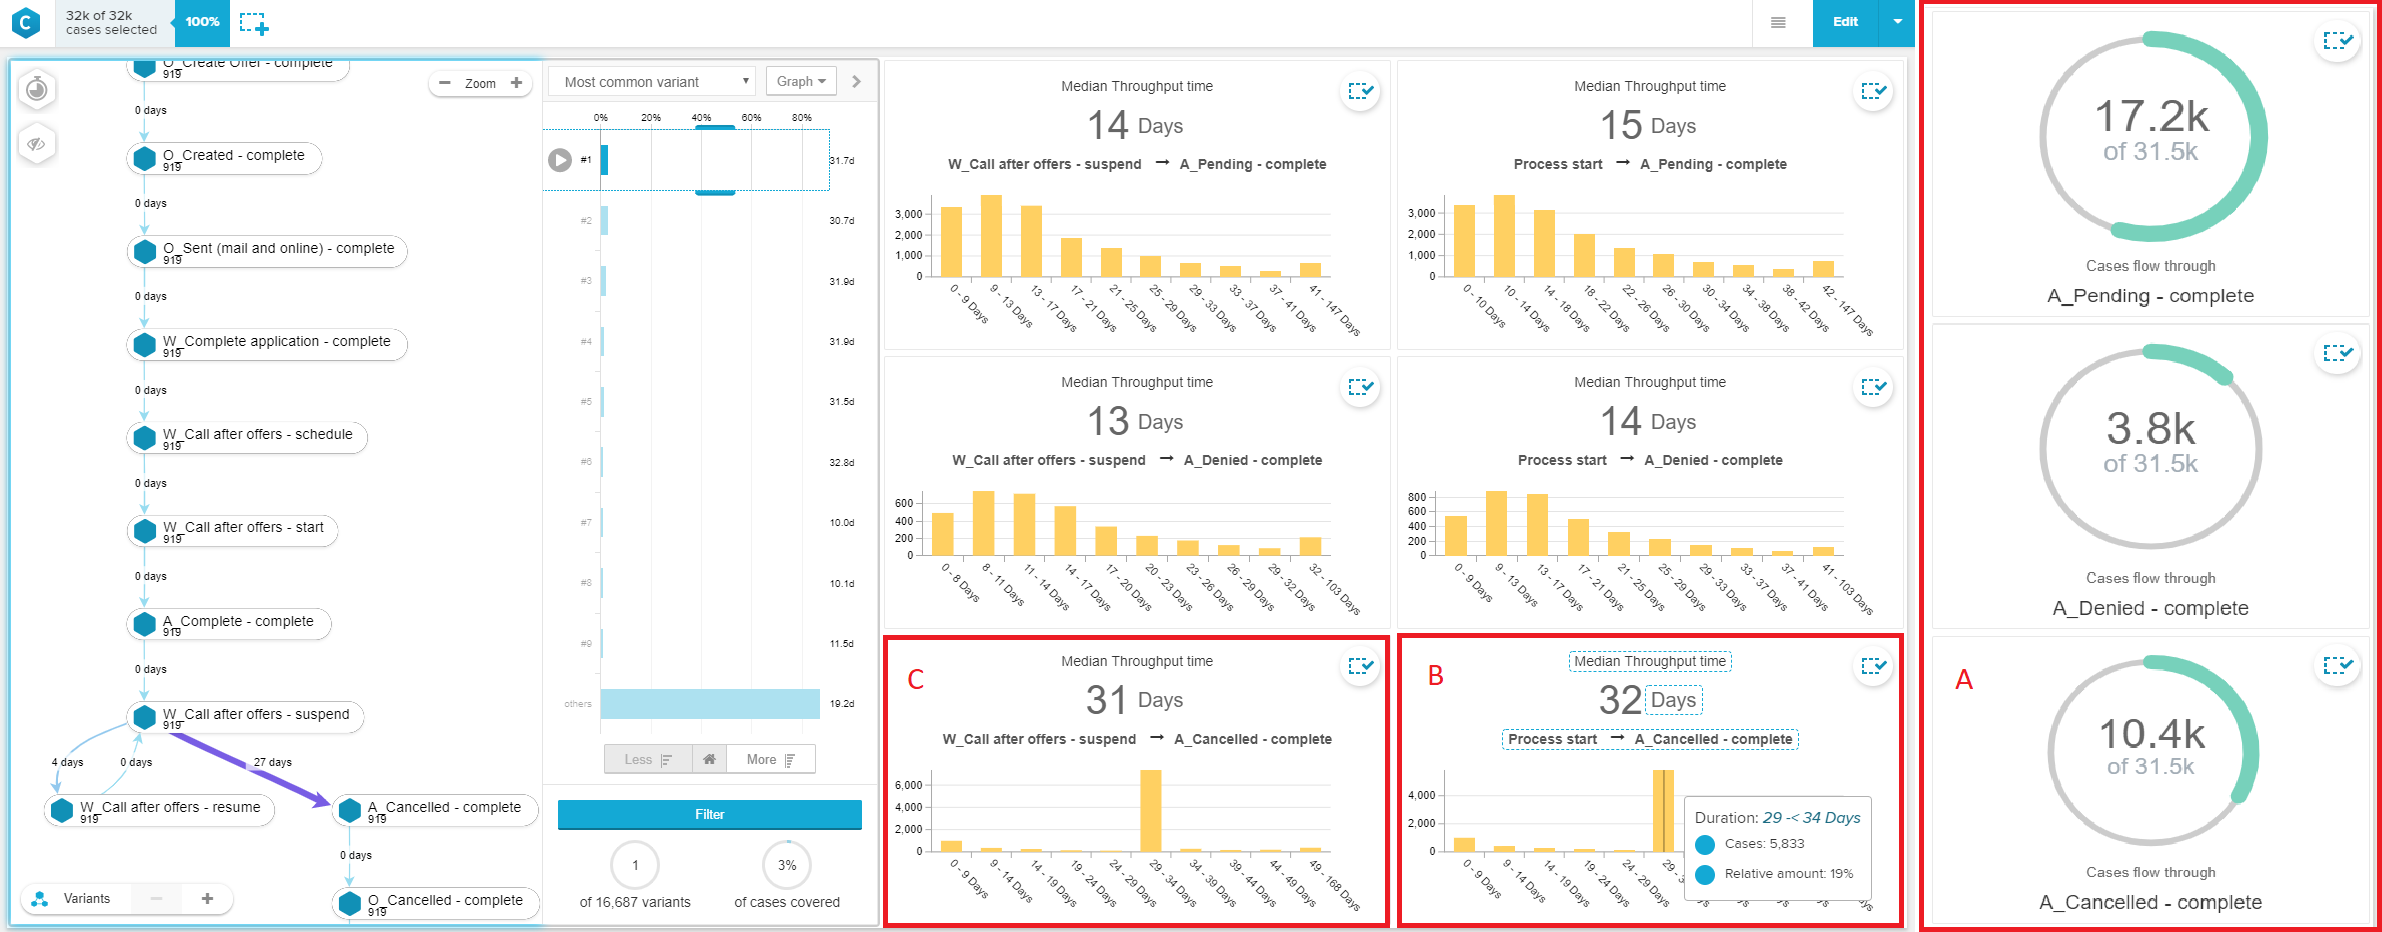
\includegraphics[width=\textwidth]{images/throughput_time.png}
\caption{\label{fig:outcome}Loan process mining in time perspective.}
\end{figure}

%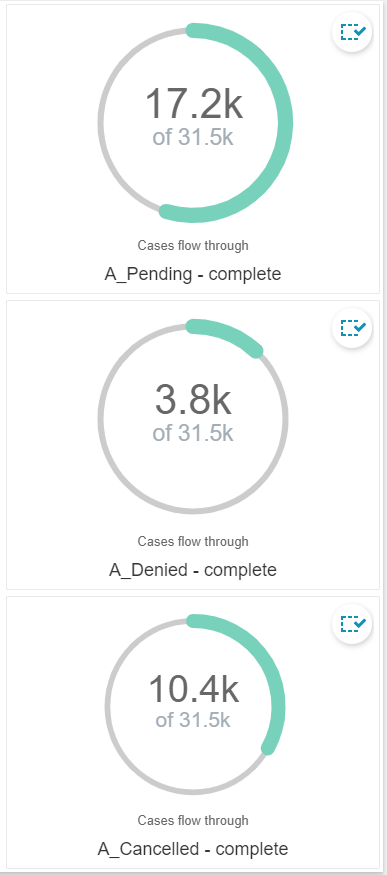
\includegraphics[width=5cm, height=10cm]{outcome}
%\begin{wrapfigure}{l}{0.9\textwidth} %this figure will be at the right
%\centering
%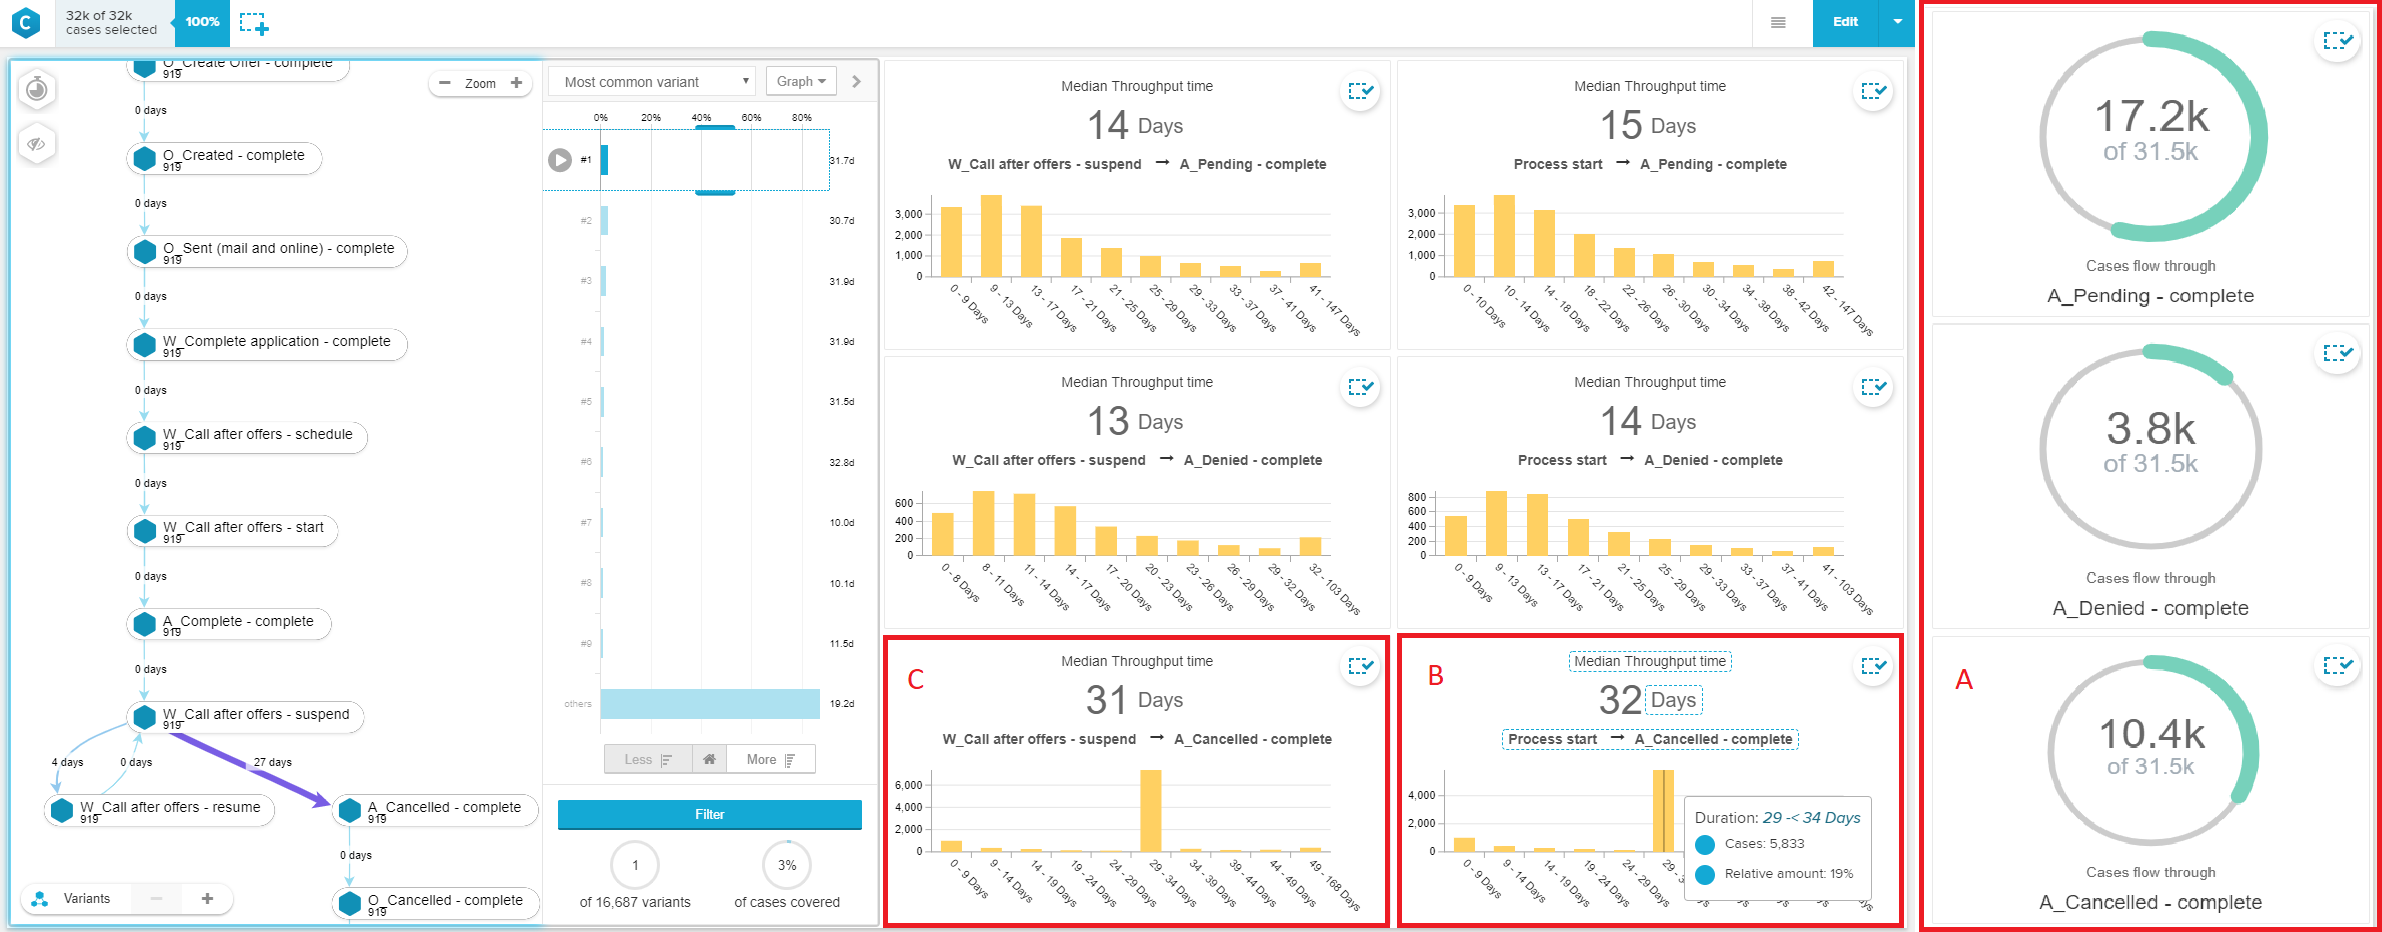
\includegraphics[width=0.25\textwidth]{images/throughput_time.png}
%\end{wrapfigure}

Our derivation affirms such questions by the financial institute about the interaction with the client and the fact of bottlenecks occurred also by the client.
Another view is equally put by the winner of the challenge\cite{winner} by dividing process flow into intervals. The process lag by client’s fault and the process lag by employee’s fault.




\section{Pre-processing log}

After over-viewing the whole process log by mining specific information within perspectives, and having some insights about what the critical parts of data to process could be, we aim to pre-process data as follows:
We use ProM platform to export XES file to CSV file to easy elaborate dataset in python environment to apply data mining techniques and further analysis.
The first step composed of cleaning log from incomplete cases since the log has been slipped in a point of time that there were some cases in phase of treatment.
(however, this step could be performed by ProM itself) but we want to assume that the final activity to consider in a case, this with one of outcome event (A\_Pending, A\_Cancelled or A\_Denied). To do so we cut case until these three events. It is important o notice the difference between to structures of log XES and CSV. XES is life cycle aware but csv is flat structure.
\begin{center}
\begin{table}[h]
\begin{tabular}{ l|c|c } 
 
 Log & Number of cases & Number of variants \\
 \hline
 Original & 31,509 & 4,047 \\ 
 
 Preprocessed & 31,194 & 3,544 \\ 


\end{tabular}
\caption{Original vs Pre-processed Log.\label{preprocessed}}\\
\end{table}
\end{center}

We find that there are 2,924 variant that contain only one case each, this make clustering methods challenging because each of these cases must -in the ideal way- considered as a unique cluster. In the other hand a cluster with one instance (case) will be non-useful and as this disadvantage we so call them difficult cases.











\begin{titlepage}
\maketitle
\end{titlepage}



% Change Bibliography to References
\renewcommand\bibname{REFERENCES}
\clearpage
\phantomsection
\addcontentsline{toc}{chapter}{REFERENCES}
\printbibliography




\end{document}

Prediction goals:  recommendation systems:
==========================================
Prediction(recommendation) is important in business process intelligence domain while day a day process running for a new applicant, this case will be evaluated by the employee as a single case without taking in account the history of similar cases. In addition, since recently hired employees do not have experience and do not understand obviously already completed case. For this reason, a prediction system would be crucial, and the profile of each case would be taken into consideration to predict a given incomplete running case.





Case study analysis:
Bank's loan process was proposed as case a study in BPIC 2017 from Dutch financial institute in The Netherlands. In such cases, certain problematics in the way how the process perform, process down time and interacting with client are challenging.
Precisely, the first question, the throughput times per part of the process,  in particular the difference between the time spent in the company's systems waiting for processing by a user and the time spent waiting on input from the applicant as this is currently unclear.(1) https://www.win.tue.nl/bpi/doku.php?id=2017:challenge
In this thesis, we will consider reports submitted from the student category.
To understand the process presented in the challenge is it useful to structure the schema in mind as follow: An application is submitted. Then, some automatic checks are performed, then generate the suitable offer to client. This offer could be sent by online or by mail. A phone discussion then is made with client about this offer and waiting him/her to confirm the offer and send additional documents and information is needed. When receiving, a validation phase to assess offer is mandatory. In case of incomplete application or missing information, the financial institute will again contact the client to add them. When completion, A series of checks should be performed after which the verdict of application is made.

Winner:
The intention for the analysis was to measure the effectiveness of system by analyzing its downtime and the density of interaction with clients.
 

NOTES:
1.	Thanks to Start timestamp and Complete timestamp to allow calculating execution time
2.	a snippet of the table
3.	our event log is a complete table in term of sparsity, since there is no sparse in case information. In contrary, there is not an important number of features / attributes for a case (4 columns), the rest of columns are event attributes that we called it meta event data not been taken in account while classifying.
4.	Textual methods Doc2vec: ScaleAbout current model uses tagging mechanism to tag the videos and the articles (“topic modeling”) and measuring distance between tags.
5.	Business process monitoring is concerned with the analysis of events produced during the execution of a process in order to assess the fulfillment of its compliance requirements and performance objectives
